So far we have shown how to implement and optimize tree reductions in CUDA.
The goal of this chapter is to investigate the properties of the optimized kernel more closely and to provide quantitative data on how the kernel performs. 
The following question will be answered:
How should the parallelisation parameters (in our case only the number of threads per block) be chosen?
How does the kernel scale with larger and smaller array sizes?
How does the underlying data type (int32, int64, float, double, complex float, complex double) affect performance?


\section{Parallelisation parameters}

\begin{figure} \label{fig_num_threads}
    \centering
    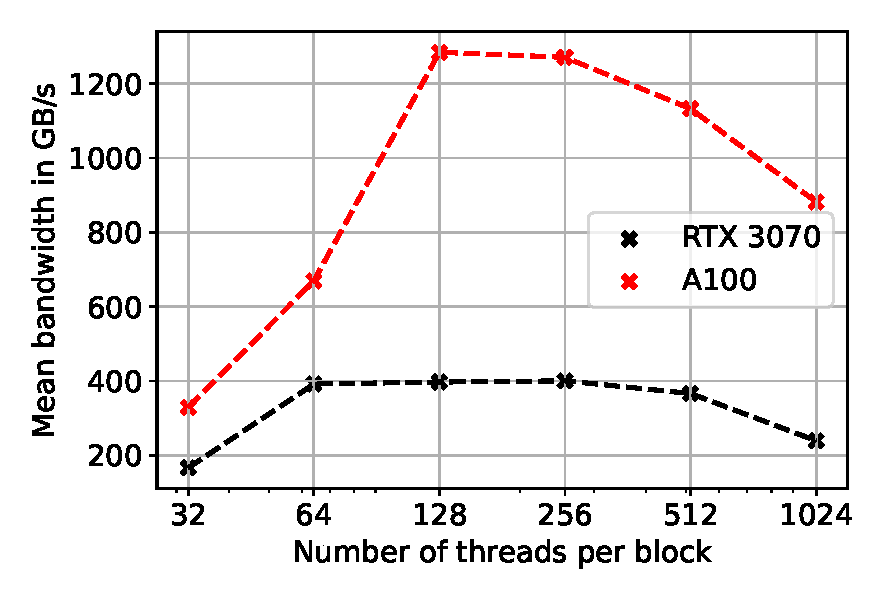
\includegraphics{num_threads.pdf}
    \caption{
        Benchmarks of the optimised kernel for \( 2^{27} \) 32-bit integers on a RTX 3070 (black) and A100 (red) for different number of threads per block.
        While the A100 outperformes the RTX 3070 as expected, they show they same characteristic in respect to the number of threads per block.
        The optimum lies somewhere between 128 and 256 threads.
    }
\end{figure}

The choice of the number of threads can have a massive impact on the performance of the application.
Usually, the optimum cannot be predicted theoretically as this becomes unfeasably complex even for simple code.
Different algorithms behave differently and it is hard to make a general statement about the optimum.
An expected behaviour, however, is the divergence for a low number of threads per block.
Here, the parallelisation overhead becomes very large and the hardware occupancy low.

The best way to approach this problem is to do test-runs of the desired calculation to find the optimum and the commit to the choice.
In our case, the optimum lies between 128 and 256 threads for both the RTX 3070 and the A100.
For the rest of the benchmarks we will therefore use 256 threads per block.

\section{Scaling of the performance towards larger and smaller array sizes}

\begin{figure} \label{fig_scaling}
    \centering
    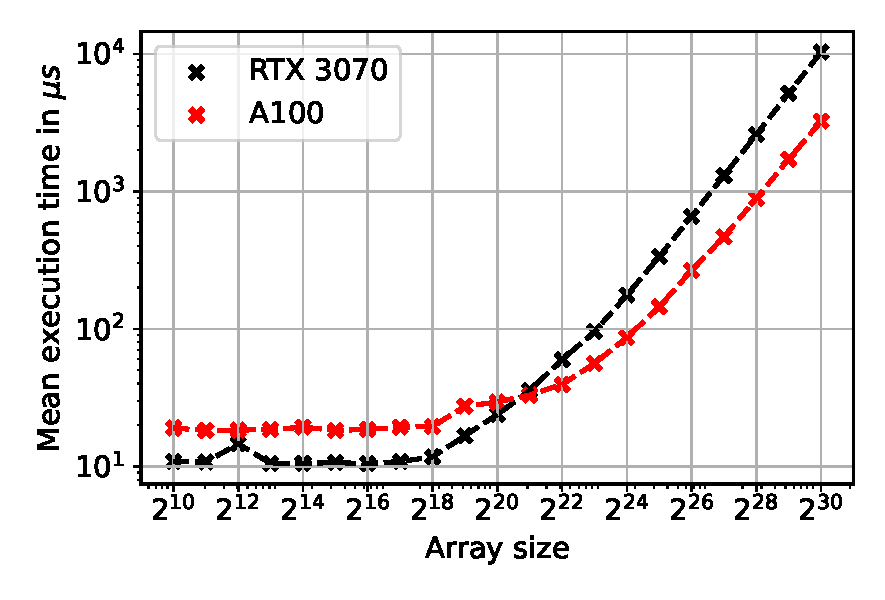
\includegraphics{scaling.pdf}
    \caption{
        Performance of the reduction kernel over increasing 32-bit array sizes for a RTX 3070 and an A100.
        All point represent the mean of 1000 measurements.
        One can see nicely the transition to linear scaling.
    }
\end{figure}

Oftentimes, the GPUs only start to be effective for large problem sizes.
This behaviour is depicted in fig. \ref{fig_scaling}.
The expected linear scaling in problem size is only achieved after a certain threshold.
The cause of this is most likely host code overhead, parallelisation overhead and device latency.
Interestingly, the RTX 3070 performs better for small array sizes.
This might be very setup dependent, however (host memory speed, CPU, etc).

Both GPUs converge towards 92\% of their respective bandwidths (RTX 3070: 448 GBytes/s, A100: 1.555 GBytes/s).
The A100 is approximately three times faster than the RTX 3070.

\section{Dependence of the performance on the datatype}

\begin{figure} \label{fig_datatypes}
    \centering
    \includegraphics{datatypes.pdf}
    \caption{
        Performance of the reduction kernel for several datatypes over an array with \( 2^{28} \) elements on a RTX 3070 (black) and an A100 (red).
        Each data point reflects the mean of 1000 measurements.
        The execution time is proportional with the size of the datatype in the case of the RTX 3070,
        while for the A100 the larger datatypes are slightly more efficient in terms of bandwidth.
    }
\end{figure}

The execution time behaviour is often times nontrivially dependent on the underlying datatype.
In our case this dependence is depicted in fig. \ref{fig_datatypes}.
In the case of the RTX 3070 the execution time is perfectly proportional to the bit size of the datatype.
This is expected as the reduction algorithm is bottlenecked by bandwidth.
Interestingly, this behaviour is not so trivial for the A100.
The A100 is slightly more efficient for the larger datatypes, int64 and double, than for the smaller ones, int32 and float.
The cause of this could be an interesting research topic for future work.

\section{Conclusion}
The most important learning from the benchmarks is that the presented implementation of tree reduction is able to achieve top performance on two different Nvidia platforms.
This shows that the optimisations have a good level of generality. 
What could not be shown is the applicability of these techniques to platforms of other GPU designers, like AMD, and could be an interesting topic for future work.
However, AMD uses a similar runtime and framework to CUDA and the GPUs have similar structure.
Therefore, one could assume that the same optimisations hold.
